\documentclass[10pt,a4paper]{amsart}
\usepackage[margin=19mm]{geometry}
\usepackage{amsmath,amssymb,mathtools}
\usepackage[scr=rsfs,cal=euler]{mathalfa}
\usepackage{xfrac}
\usepackage[unicode,hidelinks,bookmarks=false]{hyperref}
\newcommand{\ie}{i.e.\ }
\newcommand{\cf}{cf.\ }
\newcommand{\resp}{respectively\ }
\newcommand{\Subsection}{\subsection}
\providecommand{\nobreakdash}{\nobreak\hbox{-}}
\setlength{\emergencystretch}{2em}
\multlinegap0pt
\usepackage{tikz}
\usepackage{amssymb}
\usepackage[shortlabels]{enumitem}
\newtheorem{theorem}{Theorem}
\title{Total Roman bondage number of a graph}
\author{Fahimeh Khosh-Ahang Ghasr, Sakineh Nazari-Moghaddam}
\date{Source: arXiv:2602.08758v1 (CC BY 4.0)}
\begin{document}
\maketitle

\noindent\emph{Source and licence.} Total Roman bondage number of a graph. Version arXiv:2602.08758v1 (CC BY 4.0), distributed by arXiv under the Creative Commons Attribution 4.0 International licence, http://creativecommons.org/licenses/by/4.0/, as recorded in the arXiv licence metadata for this exact version and shown on the abstract page https://arxiv.org/abs/2602.08758v1. Full licence notice: \texttt{licenses/arxiv-2602.08758-CC-BY-4.0.txt}.\par\smallskip

\noindent\textit{Editorial scope.} Counted unit: the article's theorem theorem (source0.tex lines 330--332). The article's complete original proof of it is delivered with it (source0.tex lines 334--512, one \texttt{proof} environment of 179 lines). No mathematics is written, repaired or re-derived: the statement and the proof are the article's own lines, in the article's own notation, and no retained line is substituted or re-flowed.  No further source-local context is needed: every cross-reference of every retained line resolves inside the two delivered spans.  Nothing was omitted from any retained span, so the package carries no omission record.  No retained line contains a citation, so the wrapper carries no bibliography and no bibliography entry.  The retained lines contain the article's own diagram code, which the wrapper typesets with the standard tikz packages; no image file is delivered and the package declares no asset dependency.  Editorial formatting only, in addition: an AMS \texttt{amsart} preamble that restates the article's own declarations and macros used by the retained lines, namely the environments \texttt{theorem} on separate counters, together with the standard packages those lines need.  The retained environments print in this document as Theorem 1 in order of appearance, whereas the article prints the same items with the numbering of its own full document.  The complete native source of the article as distributed in the arXiv e-print for this exact version is bundled unchanged as \texttt{sources/194271/source0.tex}.
\begin{theorem}
The TR-Bondage problem is NP-hard.
\end{theorem}

\begin{proof}
Let $U=\{u_1, u_2, \dots , u_n\}$ and $\mathcal{C}%
=\{C_1, C_2, \dots , C_m\}$ be an arbitrary instance of the 3-SAT problem.
We will construct a graph $G$ and a positive integer $k$ such that $\mathcal{%
C}$ is satisfiable if and only if $b_{tR}(G)\leq k.$

\begin{figure}[ht]
\centering
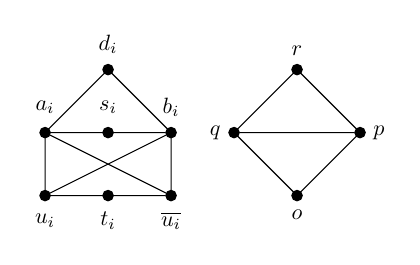
\begin{tikzpicture}[scale=.8, transform shape]
\node [draw, shape=circle,fill=black,scale=0.5] (a1) at  (0,0) {};
\node [draw, shape=circle,fill=black,scale=0.5] (a2) at  (1,0) {};
\node [draw, shape=circle,fill=black,scale=0.5] (a3) at  (2,0) {};
\node [draw, shape=circle,fill=black,scale=0.5] (a4) at  (0,1) {};
\node [draw, shape=circle,fill=black,scale=0.5] (a5) at  (1,1) {};
\node [draw, shape=circle,fill=black,scale=0.5] (a6) at  (2,1) {};
\node [draw, shape=circle,fill=black,scale=0.5] (a7) at  (1,2) {};
\draw(a1)--(a3)--(a6)--(a1)--(a4)--(a3)--(a6)--(a7)--(a4)--(a6);
\node at (0,-.4) {$u_i$};
\node at (1,-.4) {$t_i$};
\node at (2,-.4) {$\overline{u_i}$};
\node at (0,1.4) {$a_i$};
\node at (1,1.4) {$s_i$};
\node at (2,1.4) {$b_i$};
\node at (1,2.4) {$d_i$};
\node [draw, shape=circle,fill=black,scale=0.5] (a1) at  (3,1) {};
\node [draw, shape=circle,fill=black,scale=0.5] (a2) at  (4,0) {};
\node [draw, shape=circle,fill=black,scale=0.5] (a3) at  (5,1) {};
\node [draw, shape=circle,fill=black,scale=0.5] (a4) at  (4,2) {};
\draw(a1)--(a3)--(a2)--(a1)--(a4)--(a3);
\node at (2.7,1) {$q$};
\node at (5.3,1) {$p$};
\node at (4,-.3) {$o$};
\node at (4,2.3) {$r$};
\end{tikzpicture}
\caption{The graphs $H_i$ and $F$.}
\label{fig-1}
\end{figure}

For each variable $u_i\in U,$ associate the connected graph $H_{i}$ as
shown in Figure 1. Corresponding to each clause $C_{j}=\{x_j, y_j, z_j\}\in \mathcal{C}$, associate a single vertex $c_{j}$ and add the edge-set $E_j=\{c_jx_j,c_jy_j,c_jz_j\}$. Next add the graph $F$ and join
vertex $r$ to each $c_j$, and let $G$ be the resulting graph. Clearly $G$
is a graph of order $7n+m+4$ and size $10n+4m+5$.  An example of the graph $G$ when $U=\{u_1, u_2, u_3, u_4\}$ and $\mathcal{C}=\{\{u_1, u_2, \overline{u_3}\}, \{u_2, \overline{u_3}, \overline{u_4}\}\}$ is illustrated in Figure \ref{fig-2}. 

\begin{figure}[ht]
\centering
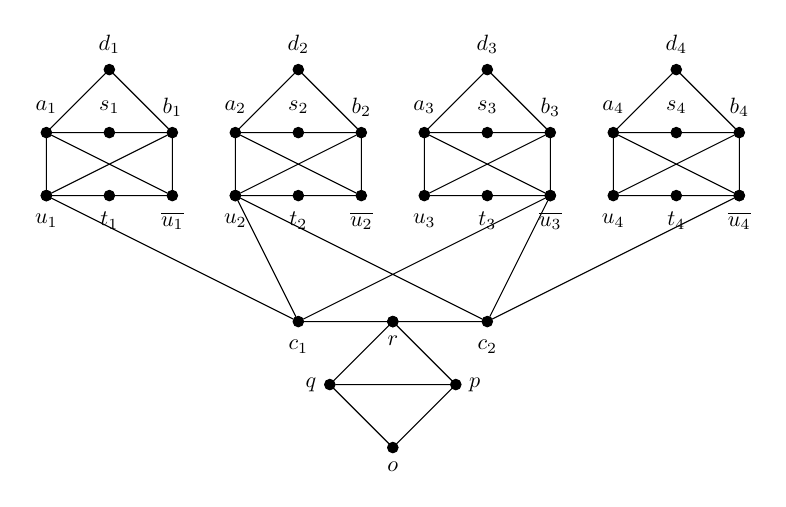
\begin{tikzpicture}[scale=.8, transform shape]
\node [draw, shape=circle,fill=black,scale=0.5] (a1) at  (0,0) {};
\node [draw, shape=circle,fill=black,scale=0.5] (a2) at  (1,0) {};
\node [draw, shape=circle,fill=black,scale=0.5] (a3) at  (2,0) {};
\node [draw, shape=circle,fill=black,scale=0.5] (a4) at  (0,1) {};
\node [draw, shape=circle,fill=black,scale=0.5] (a5) at  (1,1) {};
\node [draw, shape=circle,fill=black,scale=0.5] (a6) at  (2,1) {};
\node [draw, shape=circle,fill=black,scale=0.5] (a7) at  (1,2) {};
\draw(a1)--(a3)--(a6)--(a1)--(a4)--(a3)--(a6)--(a7)--(a4)--(a6);
\node at (0,-.4) {$u_1$};
\node at (1,-.4) {$t_1$};
\node at (2,-.4) {$\overline{u_1}$};
\node at (0,1.4) {$a_1$};
\node at (1,1.4) {$s_1$};
\node at (2,1.4) {$b_1$};
\node at (1,2.4) {$d_1$};

\node [draw, shape=circle,fill=black,scale=0.5] (a1) at  (3,0) {};
\node [draw, shape=circle,fill=black,scale=0.5] (a2) at  (4,0) {};
\node [draw, shape=circle,fill=black,scale=0.5] (a3) at  (5,0) {};
\node [draw, shape=circle,fill=black,scale=0.5] (a4) at  (3,1) {};
\node [draw, shape=circle,fill=black,scale=0.5] (a5) at  (4,1) {};
\node [draw, shape=circle,fill=black,scale=0.5] (a6) at  (5,1) {};
\node [draw, shape=circle,fill=black,scale=0.5] (a7) at  (4,2) {};
\draw(a1)--(a3)--(a6)--(a1)--(a4)--(a3)--(a6)--(a7)--(a4)--(a6);
\node at (3,-.4) {$u_2$};
\node at (4,-.4) {$t_2$};
\node at (5,-.4) {$\overline{u_2}$};
\node at (3,1.4) {$a_2$};
\node at (4,1.4) {$s_2$};
\node at (5,1.4) {$b_2$};
\node at (4,2.4) {$d_2$};

\node [draw, shape=circle,fill=black,scale=0.5] (a1) at  (6,0) {};
\node [draw, shape=circle,fill=black,scale=0.5] (a2) at  (7,0) {};
\node [draw, shape=circle,fill=black,scale=0.5] (a3) at  (8,0) {};
\node [draw, shape=circle,fill=black,scale=0.5] (a4) at  (6,1) {};
\node [draw, shape=circle,fill=black,scale=0.5] (a5) at  (7,1) {};
\node [draw, shape=circle,fill=black,scale=0.5] (a6) at  (8,1) {};
\node [draw, shape=circle,fill=black,scale=0.5] (a7) at  (7,2) {};
\draw(a1)--(a3)--(a6)--(a1)--(a4)--(a3)--(a6)--(a7)--(a4)--(a6);
\node at (6,-.4) {$u_3$};
\node at (7,-.4) {$t_3$};
\node at (8,-.4) {$\overline{u_3}$};
\node at (6,1.4) {$a_3$};
\node at (7,1.4) {$s_3$};
\node at (8,1.4) {$b_3$};
\node at (7,2.4) {$d_3$};

\node [draw, shape=circle,fill=black,scale=0.5] (a1) at  (9,0) {};
\node [draw, shape=circle,fill=black,scale=0.5] (a2) at  (10,0) {};
\node [draw, shape=circle,fill=black,scale=0.5] (a3) at  (11,0) {};
\node [draw, shape=circle,fill=black,scale=0.5] (a4) at  (9,1) {};
\node [draw, shape=circle,fill=black,scale=0.5] (a5) at  (10,1) {};
\node [draw, shape=circle,fill=black,scale=0.5] (a6) at  (11,1) {};
\node [draw, shape=circle,fill=black,scale=0.5] (a7) at  (10,2) {};
\draw(a1)--(a3)--(a6)--(a1)--(a4)--(a3)--(a6)--(a7)--(a4)--(a6);
\node at (9,-.4) {$u_4$};
\node at (10,-.4) {$t_4$};
\node at (11,-.4) {$\overline{u_4}$};
\node at (9,1.4) {$a_4$};
\node at (10,1.4) {$s_4$};
\node at (11,1.4) {$b_4$};
\node at (10,2.4) {$d_4$};

\node [draw, shape=circle,fill=black,scale=0.5] (a1) at  (4,-2) {};
\node [draw, shape=circle,fill=black,scale=0.5] (a2) at  (7,-2) {};
\node [draw, shape=circle,fill=black,scale=0.5] (a3) at  (0,0) {};
\node [draw, shape=circle,fill=black,scale=0.5] (a4) at  (3,0) {};
\node [draw, shape=circle,fill=black,scale=0.5] (a5) at  (8,0) {};
\node [draw, shape=circle,fill=black,scale=0.5] (a6) at  (11,0) {};
\node [draw, shape=circle,fill=black,scale=0.5] (a7) at  (5.5,-2) {};
\draw(a3)--(a1)--(a4)--(a2)--(a5)--(a1);
\draw(a6)--(a2)--(a7)--(a1);
\node at (4,-2.4) {$c_1$};
\node at (7,-2.4) {$c_2$};

\node [draw, shape=circle,fill=black,scale=0.5] (a1) at  (4.5,-3) {};
\node [draw, shape=circle,fill=black,scale=0.5] (a2) at  (5.5,-4) {};
\node [draw, shape=circle,fill=black,scale=0.5] (a3) at  (6.5,-3) {};
\node [draw, shape=circle,fill=black,scale=0.5] (a4) at  (5.5,-2) {};
\draw(a1)--(a3)--(a2)--(a1)--(a4)--(a3);
\node at (4.2,-3) {$q$};
\node at (6.8,-3) {$p$};
\node at (5.5,-4.3) {$o$};
\node at (5.5,-2.3) {$r$};
\end{tikzpicture}
\caption{An example of the graph $G$.}
\label{fig-2}
\end{figure}

Set $k=1$. Note that for every $\gamma _{tR}(G)$-function $f=(V_0, V_1, V_2)$, we
have $f(V(H_i))\geq 4$ for each $i\in \{1,2,\dots ,n\}$ and $f(V(F))\geq 3$. Therefore $\gamma _{tR}(G)\geq 4n+3$.\newline
\newline
\textbf{Claim 1.} $\gamma _{tR}(G)=4n+3$ if and only if $\mathcal{C}$ is satisfiable.\newline
\textit{Proof of Claim 1.} Assume that $\gamma _{tR}(G)=4n+3$ and let $f=(V_0, V_1, V_2)$ be a $\gamma _{tR}(G)$-function. Then $f(V(H_i))=4$ for each $i\in \{1,2,\dots ,n\}, f(V(F))=3$  and the value of $f$ on other vertices is zero. More precisely, $f(V(F))=3$ implies that $f(r)=1,f(o)=0$ and either ($f(p)=2$ and $f(q)=0$) or ($f(p)=0$ and $f(q)=2$). Moreover, $f(V(H_i))=4$ implies that $\left\vert V(H_i)\cap V_2\right\vert =2$ and $\left\vert V(H_i)\cap V_1\right\vert =0$ and thus we must have either $u_i,b_i\in V_2$ or
$\overline{u_i},a_i\in V_2$. Consequently, for each $i \in \{1, \dots , n\}$ we have $\left\vert \{u_i,\overline{u_i}\}\cap V_2\right\vert =1$. Now for every $j\in\{1, 2, \dots , m\}$, since $f(c_j)=0$ and $r\notin V_2$, we deduce that  $N(c_j)\cap \{u_i,\overline{u_i}\}\neq \emptyset $ for some $i\in \{1,2,\dots ,n\}$. Let $t:U\longrightarrow \{T,F\}$ be a mapping defined by $t(u_i)=T$ if $f(u_i)=2$ and $t(u_i)=F$ if $f(\overline{u_i})=2$.
Assume that $f(u_i)=2$ and $c_j\in N(u_i)$. By the construction of $G$, the literal $u_i$ is in the clause $C_j$. Then $t(u_i)=T$, implies that the clause $C_j$ is satisfied by $t$. Next assume that $f(\overline{u_i})=2$ and $c_j\in N(\overline{u_i})$. By the construction of $G$, the literal $\overline{u_i}$ is in the clause $C_j$. Then $t(u_i)=F$ and thus $t$ assigns $\overline{u_i}$ the true value $T$. Hence $t$ satisfies the clause $C_j$ and therefore $\mathcal{C}$ is satisfiable.

Conversely, assume that $\mathcal{C}$ is satisfiable, and let $t:U\longrightarrow \{T,F\}$ be a satisfying truth assignment for $\mathcal{C}$. We construct a TRDF $h$ on $G$ as follows. For every $i \in \{1, 2, \dots , n\}$ if $t(u_i)=T$, then let $h(u_i)=h(b_i)=2$, and if $t(u_i)=F$, then let $h(\overline{u_i})=h(a_i)=2$. Also, let $h(p)=2, h(r)=1$ and $h(x)=0$
for all remaining vertices. It is easy to check that $h$ is a TRDF on $G$ of weight $4n+3$. Thus $\gamma _{tR}(G)=4n+3$ and the proof of Claim 1 is complete.\newline
\newline
\textbf{Claim 2.} For every edge $e$ of $G$, $\gamma _{tR}(G-e)\leq 4n+4$.
\newline
\textit{Proof of Claim 2.} Let $e$ be an edge of $G$. If $e\in E(H_{i})$ for some $i\in \{1,2,\dots ,n\}$, define the function $g:V(G)\longrightarrow \{0,1,2\}$ by $g(r)=g(p)=2, g(u_\ell)=g(b_\ell)=2$ for every $\ell \in \{1,2,\dots ,n\}-\{i\}$.
Now if $e\in \{a_id_i, a_is_i, a_i\overline{u_i}, t_i\overline{u_i}\}$, then let $g(u_i)=g(b_i)=2$. If $e\in \{b_id_i, b_is_i, b_iu_i, t_iu_i\}$, then let $g(a_i)=g(\overline{u_i})=2$. If $e=a_iu_i$, then $g(\overline{u_i})=g(b_i)=2$ and eventually if $e=b_i\overline{u_i}$, then let $g(u_i)=g(a_i)=2$. (Of course notice that the cases $e\in \{b_id_i, a_id_i, a_iu_i, b_i\overline{u_i}\}$ can be included in other cases.)
Any remaining vertex of $G$ is assigned a $0$ under $g$. Clearly, $g$ is a TRDF on $G-e$ of weight $4n+4$. For the next, we assume that $e\notin E(H_{i})$ for every $i\in
\{1,2,\dots ,n\}$. If $e\in E(F)$, define the function $g:V(G)\longrightarrow \{0,1,2\}$ by $g(r)=g(u_{i})=g(b_{i})=2$ for every
$i\in \{1,2,\dots ,n\}$ and if $e\in \{rp, op\}$, then let $g(q)=2$ and else let $g(p)=2$. Also $g(x)=0$ for other vertices $x$ in $G$. Clearly, $g$ is a TRDF on $G-e$ of weight $4n+4$. Assume that
$e=rc_j$ for some $j\in \{1,2,\dots ,m\}$. Then since there exists $i\in \{1,2,\dots ,n\}$
such that $N(c_j)\cap \{u_i,\overline{u_i}\}\neq \emptyset$, without
loss of generality, let $c_ju_i\in E(G)$. Then assigning a $2$ to $r,p$
and every $u_i$ and $b_i$, and a $0$ to all remaining vertices provides
a TRDF on $G-e$ of weight $4n+4$. Finally, if $e$ is an edge linking
some $c_j$ with a variable of $U$, then the previous function is
TRDF on $G-e$ of weight $4n+4$. In any case, $\gamma _{tR}(G-e)\leq
4n+4$ and the proof of Claim 2 is complete.\newline
\newline
\textbf{Claim 3.} $\gamma _{tR}(G)=4n+3$ if and only if $b_{tR}(G)=1.$
\newline
\textit{Proof of Claim 3.} Assume that $\gamma _{tR}(G)=4n+3$. Let $f=(V_0, V_1, V_2)$ be a $\gamma _{tR}(G-e)$-function, where $e=pq$. Let $F'$ be the cycle $C_4$ induced by $o,p,q$ and $r$ in $G-e$.
Clearly, $f(V(H_i))\geq 4$ and so the total weight assigned for vertices
of all $H_i$'s equals to at least $4n$. Moreover, to total Roman dominate
vertices of $F'$, we need that $f(V(F'))+\overset{m}{\underset{j=1}{\sum }}f(c_j)\geq 4$ and thus $\gamma _{tR}(G-e)\geq 4n+4$. Therefore $b_{tR}(G)=1$.

Conversely, assume that $b_{tR}(G)=1$ and let $e$ be an edge of $G$ such
that $\gamma _{tR}(G-e)>\gamma _{tR}(G)$. By Claim 2, $\gamma _{tR}(G-e)\leq
4n+4$ and since $\gamma _{tR}(G)\geq 4n+3$ we deduce that $\gamma_{tR}(G)=4n+3$ which completes the proof of Claim 3.

According to Claims 1 and 3, we obtain that $b_{tR}(G)=1$ if and only if
there is a truth assignment for $U$ that satisfies all the clauses in $\mathcal{C}$. Since the construction of the total Roman bondage instance is straightforward from a 3-SAT instance, the size of the total Roman bondage
instance is bounded above by a polynomial function of the size of 3-SAT
instance. Consequently, we obtain a polynomial transformation.
\end{proof}

\end{document}
